\documentclass[aspectratio=169, 11pt]{beamer}

% Packages
\usepackage[utf8]{inputenc}
\usepackage{amsmath, amssymb, amsfonts}
\usepackage{graphicx}
\usepackage{booktabs}
\usepackage{ragged2e}
\usepackage{minted}
\usepackage{xcolor}
\usepackage{tikz}
\usepackage{algorithm}
\usepackage{algorithmic}
\usepackage{listings}
\usepackage{tcolorbox}

\usetikzlibrary{arrows.meta,positioning,fit,shapes.symbols}
\usetikzlibrary{arrows,shapes}
\definecolor{LightGray}{gray}{0.975}
\definecolor{links}{HTML}{2A1B81}
\hypersetup{colorlinks,linkcolor=,urlcolor=blue}
\AtBeginEnvironment{minted}{%
    \renewcommand{\fcolorbox}[4][]{#4}
}

\title[SVM]{ML101 \\ Chapter 09: Support Vector Machines}
\subtitle{An Introduction to Statistical Learning, ISLRv2}
\author{James, Witten, Hastie \& Tibshirani}
\date{\today}

% Remove navigation symbols
\setbeamertemplate{navigation symbols}{}

\defbeamertemplate*{footline}{shadow theme}{
    \leavevmode
    \hbox{
        \begin{beamercolorbox}[
                wd =        0.33\paperwidth,
                ht =        2.5ex,
                dp =        1.125ex,
                leftskip =  0.3cm plus1fil,
                rightskip = 0.3cm
            ]{author in head/foot}
            \flushleft ML101
        \end{beamercolorbox}
        \begin{beamercolorbox}[
                wd =        0.33\paperwidth,
                ht =        2.5ex,
                dp =        1.125ex,
                leftskip =  0.3cm plus1fil,
                rightskip = 0.3cm
            ]{author in head/foot}
            \insertshorttitle
        \end{beamercolorbox}
        \begin{beamercolorbox}[
                wd =        0.33\paperwidth,
                ht =        2.5ex,
                dp =        1.125ex,
                leftskip =  0.3cm plus1fil,
                rightskip = 0.3cm
            ]{title in head/foot}
            \hfill \insertframenumber\,/\,\inserttotalframenumber%
        \end{beamercolorbox}
    }
}

\AtBeginSection[]
{
     \begin{frame}<beamer>
     \frametitle{Plan}
     \tableofcontents[currentsection]
     \end{frame}
}

\usefonttheme{serif}

\newcommand\Wider[2][18mm]{%
    \makebox[\linewidth][c]{%
        \begin{minipage}{\dimexpr\textwidth+#1\relax}
            \raggedright#2
        \end{minipage}%
    }%
}
\newcommand\userinput[1]{\textbf{#1}}

\begin{document}

\frame{\titlepage}

\begin{frame}{An Introduction to Statistical Learning with Applications in R}{a.k.a. ISLR}
    \centering
    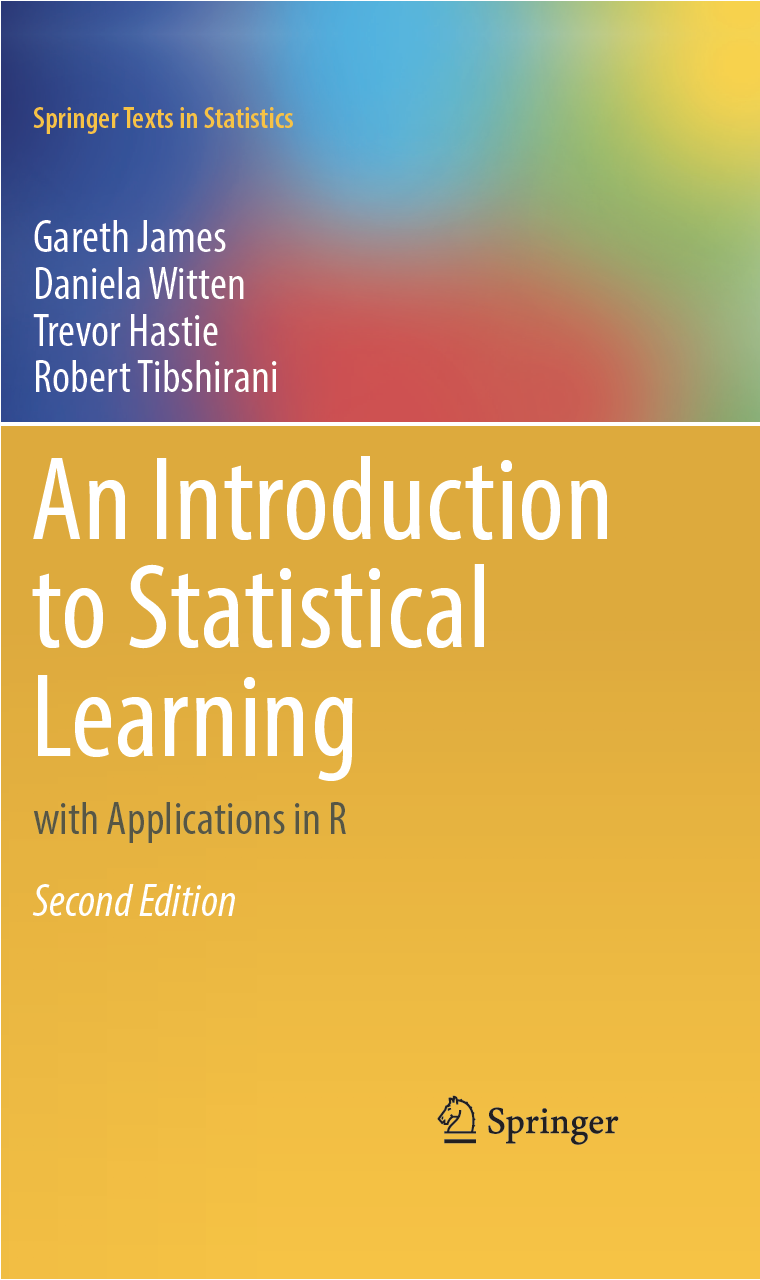
\includegraphics[height=0.7\textheight]{figures/book_cover} \\
    \vspace{4mm}
    {
        \tiny
        Content has been extracted from \textit{An Introduction to Statistical Learning with Applications in R}, Second Edition, by James, Witten, Hastie \& Tibshirani. Springer. 2023.\\
        Visit \url{https://www.statlearning.com/}.\\
    }
\end{frame}

% Slide 1
\begin{frame}{Support Vector Machines}
    Here we approach the two-class classification problem in a direct way: \\
    \vspace{1em}
    We try and find a plane that separates the classes in feature space. \\
    \vspace{1em}
    If we cannot, we get creative in two ways:
    \begin{itemize}
        \item We soften what we mean by ``separates'', and
        \item We enrich and enlarge the feature space so that separation is possible.
    \end{itemize}
\end{frame}

% Slide 2
\begin{frame}{What is a Hyperplane?}
    \begin{itemize}
        \item A hyperplane in $p$ dimensions is a flat affine subspace of dimension $p-1$.
        \item In general the equation for a hyperplane has the form
        \[ \beta_{0} + \beta_{1}X_{1} + \beta_{2}X_{2} + \dots + \beta_{p}X_{p} = 0 \]
        \item In $p=2$ dimensions a hyperplane is a line.
        \item If $\beta_{0}=0$, the hyperplane goes through the origin, otherwise not.
        \item The vector $\beta = (\beta_{1}, \beta_{2}, \dots, \beta_{p})$ is called the normal vector - it points in a direction orthogonal to the surface of a hyperplane.
    \end{itemize}
\end{frame}

% Slide 3
\begin{frame}{Hyperplane in 2 Dimensions}
    \begin{columns}[c]
    \begin{column}{0.59\textwidth}
        \centering
        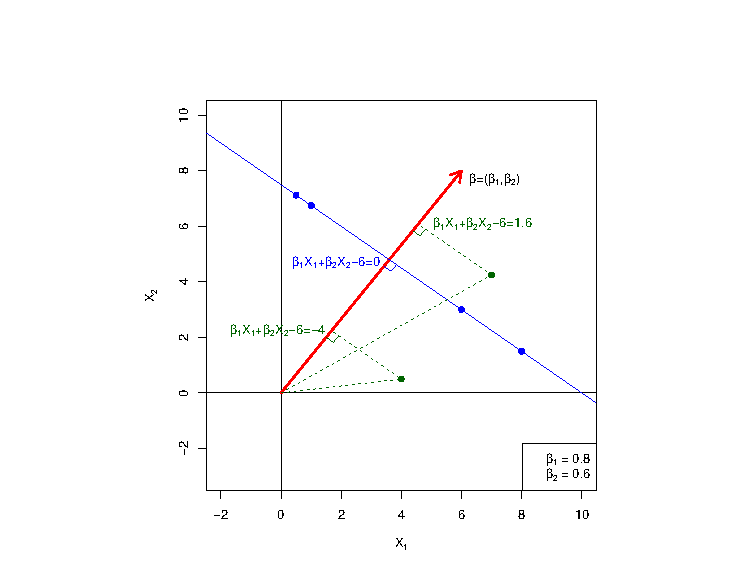
\includegraphics[width=0.8\textwidth]{figures/hp} \\
        \textit{\tiny A 2D plot illustrating a separating hyperplane (blue line) with normal vector $\beta$ (red arrow) and equations for boundaries.}
    \end{column}
    \begin{column}{0.39\textwidth}
        \begin{center}
            \footnotesize
            $\beta_{1}X_{1} + \beta_{2}X_{2} - 6 = 0$ \\
            $\beta_{1}X_{1} + \beta_{2}X_{2} - 6 = -4$ \\
            $\beta_{1}X_{1} + \beta_{2}X_{2} - 6 = 1.6$ \\
            $\beta = (\beta_{1}, \beta_{2})$, with $\beta_{1} = 0.8, \beta_{2} = 0.6$
        \end{center}
    \end{column}
    \end{columns}
\end{frame}

\begin{frame}{Separating Hyperplanes}
    \centering
    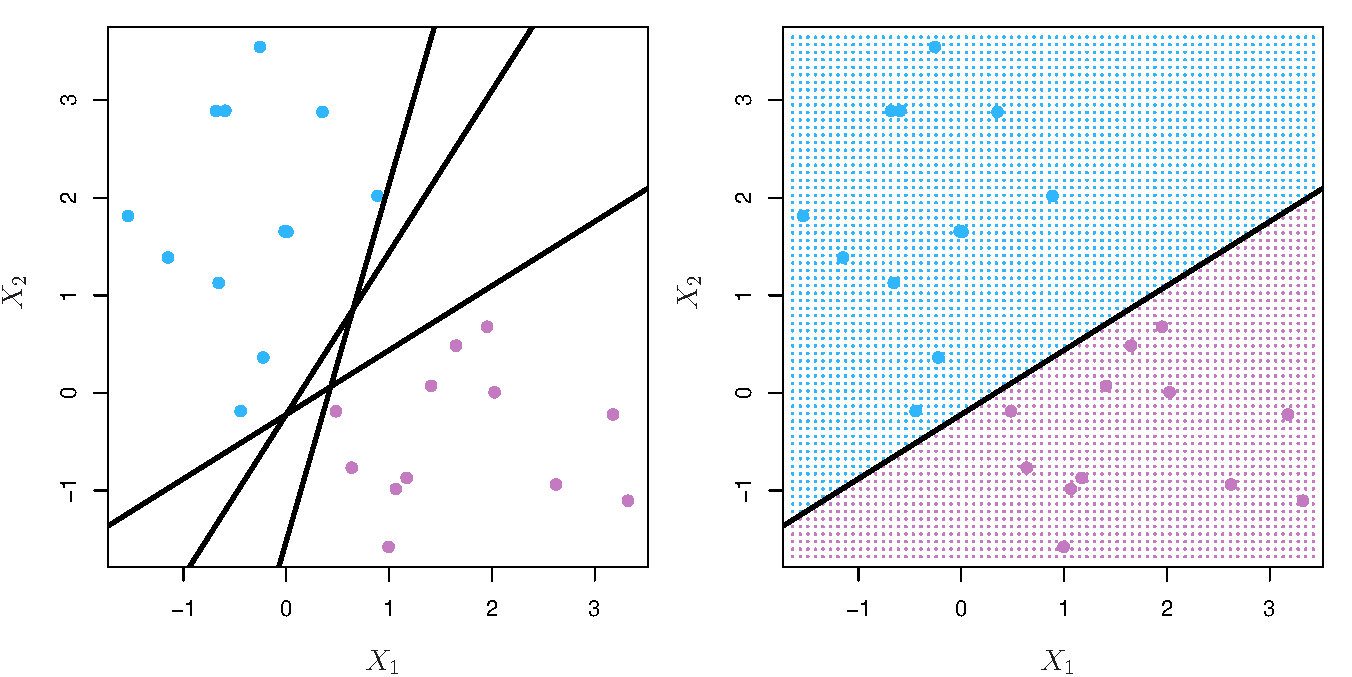
\includegraphics[width=0.8\textwidth]{figures/9_2} \\
    \vspace{-2mm}
    \textit{\tiny Linearly separable data with multiple potential separating hyperplanes. The margin of classification shaded in blue and pink.}
    \begin{itemize}
        \footnotesize
        \item If $f(X) = \beta_{0} + \beta_{1}X_{1} + \dots + \beta_{p}X_{p}$ then $f(X) > 0$ for points on one side of the hyperplane, and $f(X) < 0$ for points on the other.
        \item If we code the colored points as $Y_{i} = +1$ for blue, say, and $Y_{i} = -1$ for mauve, then if $Y_{i} \cdot f(X_{i}) > 0$ for all $i$, $f(X) = 0$ defines a separating hyperplane.
    \end{itemize}
\end{frame}

\begin{frame}{Maximal Margin Classifier}
    \begin{columns}[c]
        \begin{column}{0.49\textwidth}
            \centering
            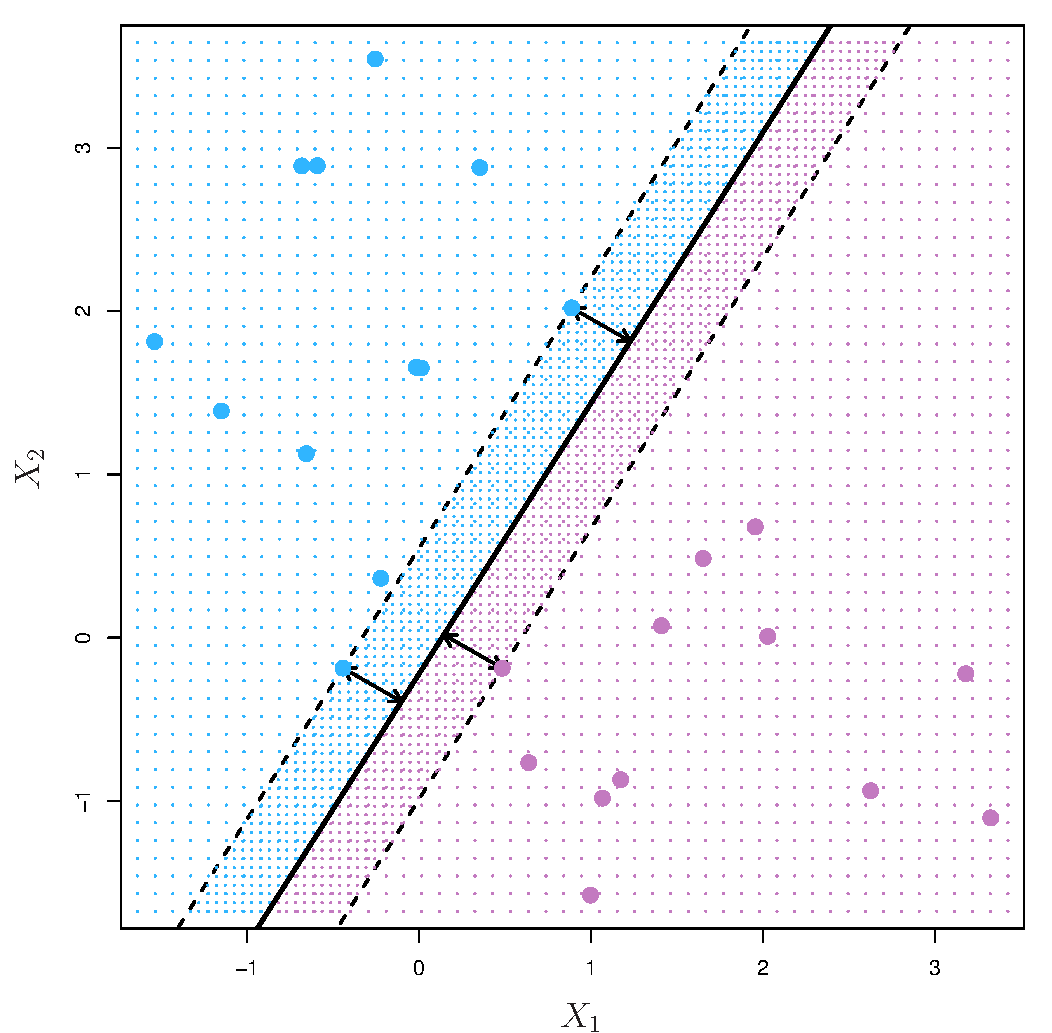
\includegraphics[width=0.9\textwidth]{figures/9_3} \\
            \textit{\tiny A 2D plot showing the maximal margin classifier. The margin is maximized between the two classes with arrows pointing to the support vectors.}
        \end{column}
        \begin{column}{0.49\textwidth}
            \footnotesize
            Among all separating hyperplanes, find the one that makes the biggest gap or margin between the two classes.\\
            Constrained optimization problem:
            $$\underset{\beta_{0},\beta_{1},\dots,\beta_{p}}{\text{maximize}}\; M$$
            subject to
            $$\sum_{j=1}^{p}\beta_{j}^{2} = 1,$$
            $$y_{i}(\beta_{0} + \beta_{1}x_{i1} + \dots + \beta_{p}x_{ip}) \ge M$$
            for all $i=1,\dots,N$ \\

            \vspace{3mm}
            \pause
            This can be rephrased as a convex quadratic program, and solved efficiently. The function \texttt{svm()} in package \texttt{e1071} solves this problem efficiently.
        \end{column}
    \end{columns}
\end{frame}

\begin{frame}{Non-separable Data}
    \begin{columns}
        \begin{column}{0.6\textwidth}
            \centering
            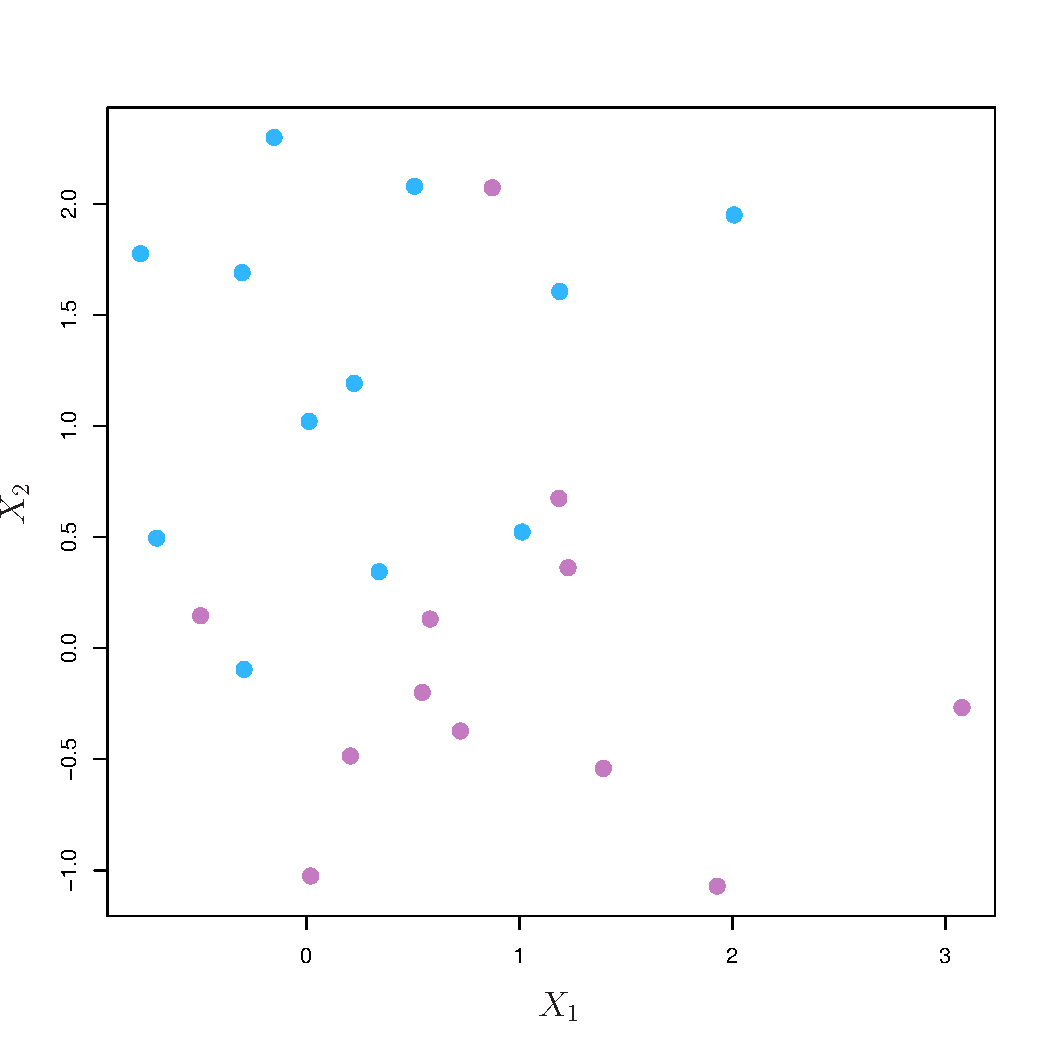
\includegraphics[width=0.7\textwidth]{figures/9_4} \\
            \textit{\tiny A scatterplot showing non-separable classes where blue and mauve points are intermixed.}
        \end{column}
        \begin{column}{0.4\textwidth}
            The data on the left are not separable by a linear boundary. \\
            \vspace{3mm}
            This is often the case, unless $N < p$.
        \end{column}
    \end{columns}
\end{frame}

\begin{frame}{Noisy Data}
    \centering
    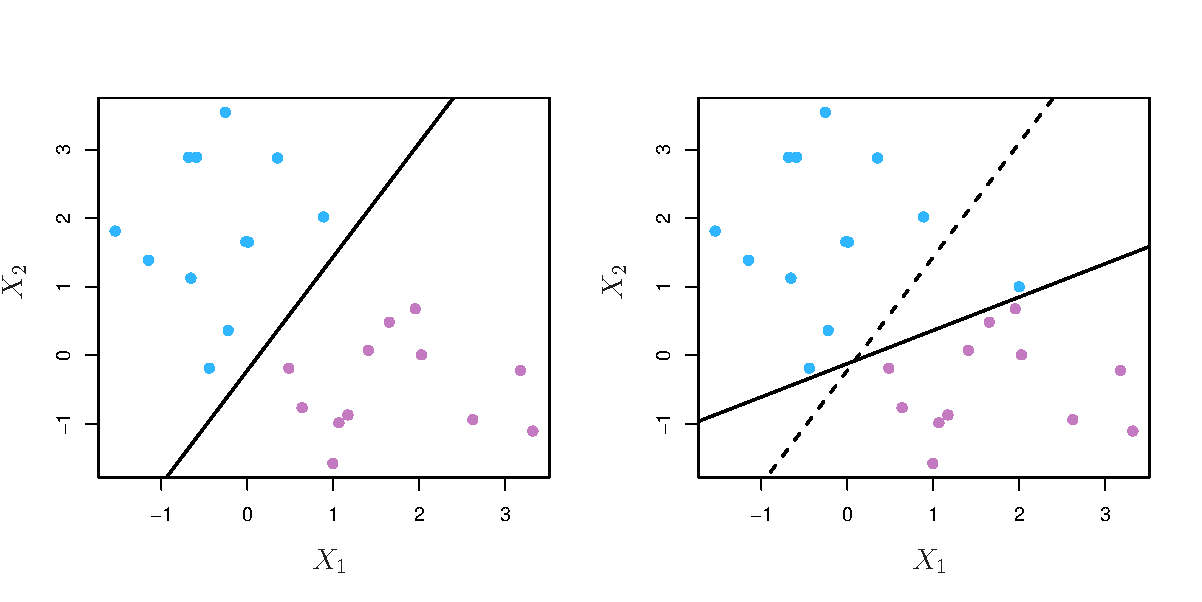
\includegraphics[width=\textwidth]{figures/9_5} \\
    \vspace{-2mm}
    Sometimes the data are separable, but noisy. This can lead to a poor solution for the maximal-margin classifier. \\
    \pause
    \vspace{1mm}
    The support vector classifier maximizes a soft margin.
\end{frame}

\begin{frame}{Support Vector Classifier}
    \centering
    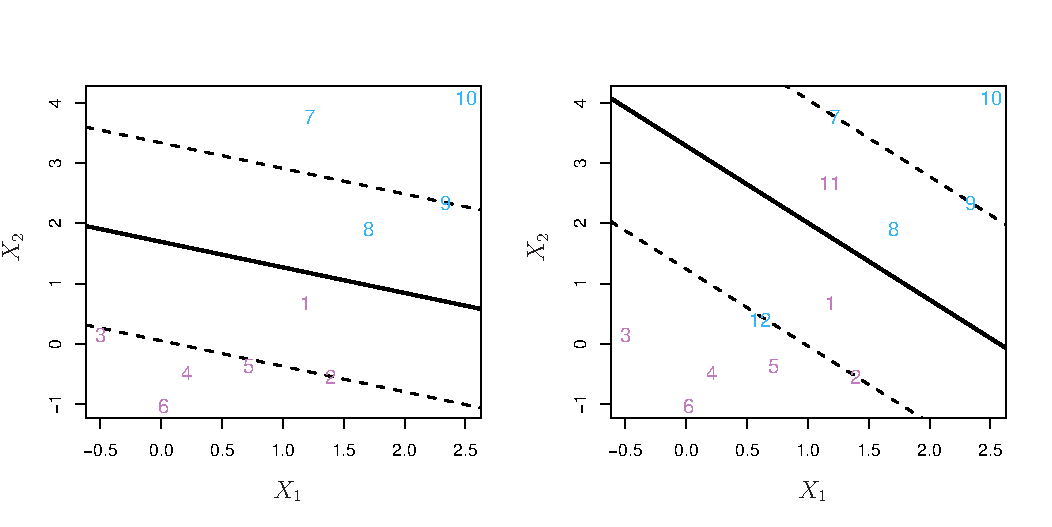
\includegraphics[width=0.9\textwidth]{figures/9_6} \\
    \vspace{-2mm}
    \textit{\tiny Plots demonstrating a soft margin classifier. Numbers identifies support vectors, some of which fall within the the wrong side.} \\
    \vspace{1mm}
    $\underset{\beta_{0},\beta_{1},\dots,\beta_{p},\epsilon_{1},\dots,\epsilon_{n}}{\text{maximize}}\; M$ \quad subject to $\sum_{j=1}^{p}\beta_{j}^{2} = 1,$ \\
    $y_{i}(\beta_{0} + \beta_{1}x_{i1} + \beta_{2}x_{i2} + \dots + \beta_{p}x_{ip}) \ge M(1 - \epsilon_{i}),$ \\
    $\epsilon_{i} \ge 0, \quad \sum_{i=1}^{n}\epsilon_{i} \le C$
\end{frame}

\begin{frame}{Support Vector Classifier}
    \centering
    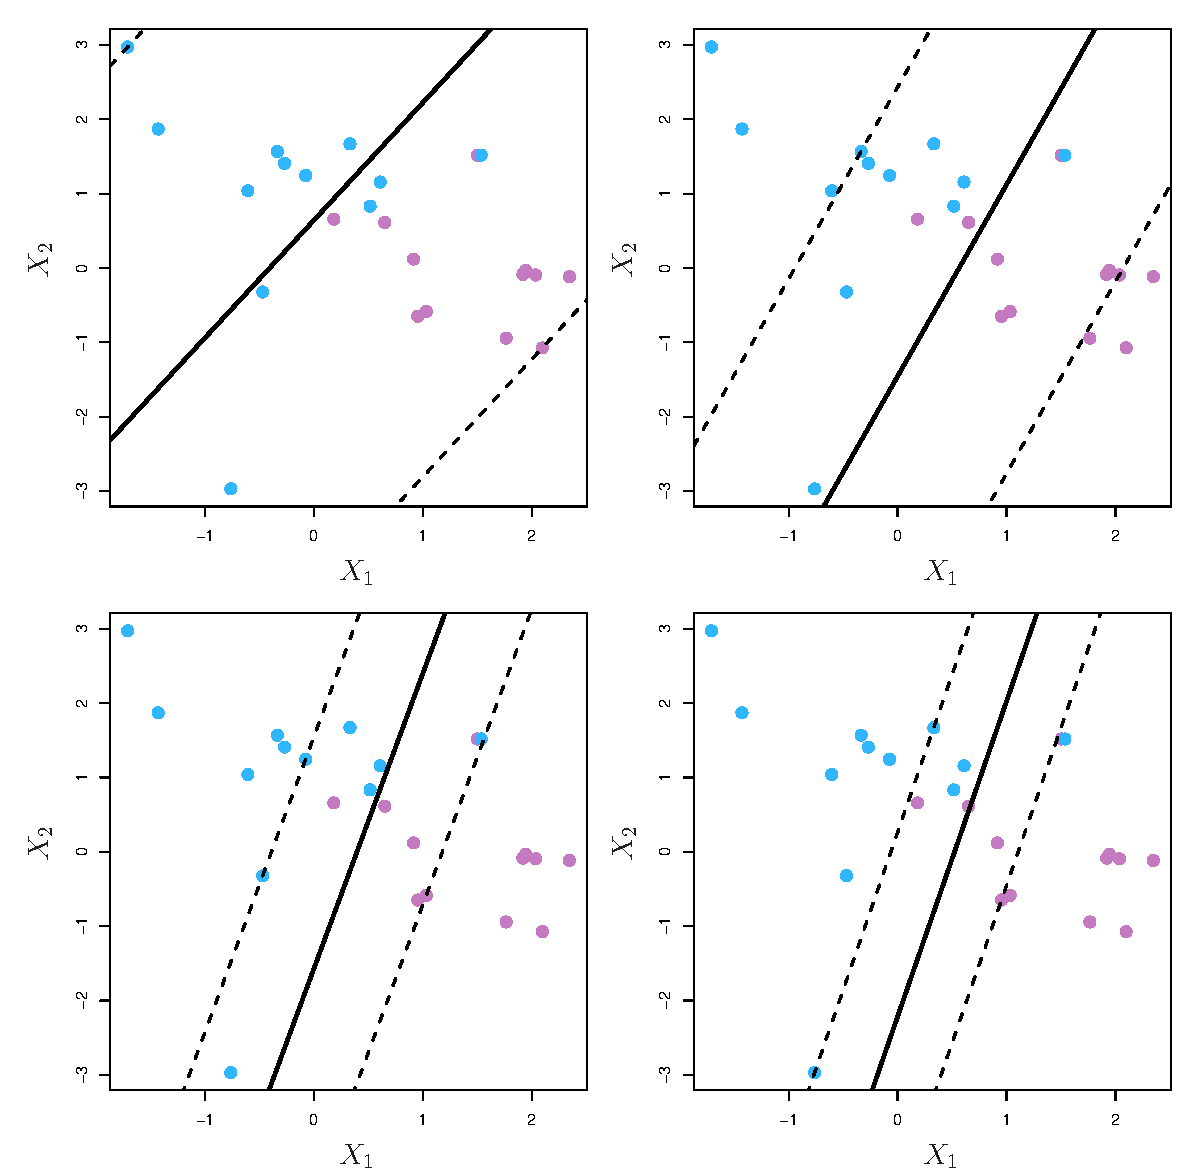
\includegraphics[width=0.5\textwidth]{figures/9_7} \\
    \textit{\tiny The effect of varying the regularization parameter C on the soft margin width and decision boundary.} \\
    \begin{itemize}
        \item C is a regularization parameter.
    \end{itemize}
\end{frame}

\begin{frame}{Linear boundary can fail}
    \begin{columns}
        \begin{column}{0.6\textwidth}
            \centering
            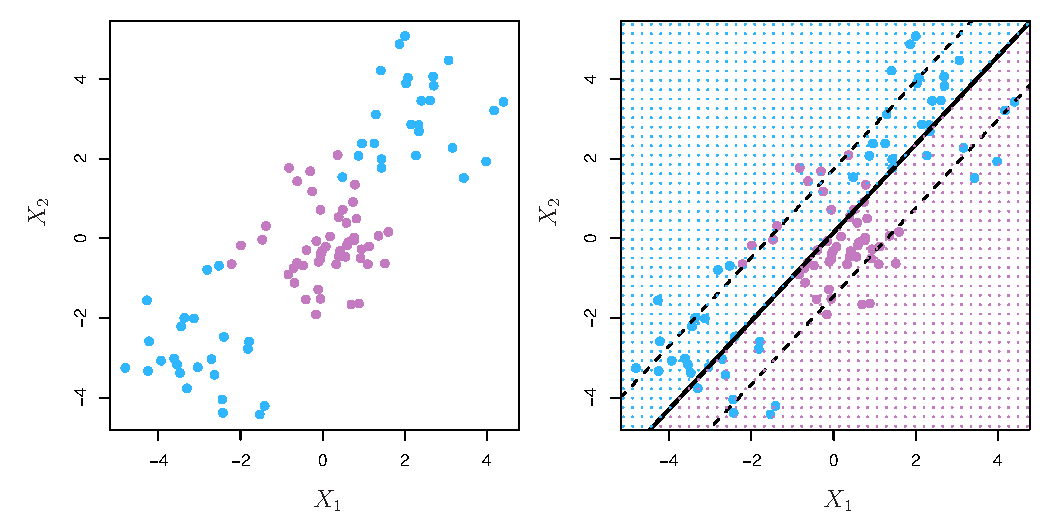
\includegraphics[trim={0cm 0cm 9cm 0cm}, clip, width=0.8\textwidth]{figures/9_8} \\
            \textit{\tiny One class concentrated in the center and the other distributed around it.}
        \end{column}
        \begin{column}{0.4\textwidth}
            Sometime a linear boundary simply won't work, no matter what value of C. \\
            \vspace{1mm}
            The example on the left is such a case. \\
            \vspace{1mm}
            What to do?
        \end{column}
    \end{columns}
\end{frame}

\begin{frame}{Linear boundary can fail}
    \begin{columns}
        \begin{column}{0.6\textwidth}
            \centering
            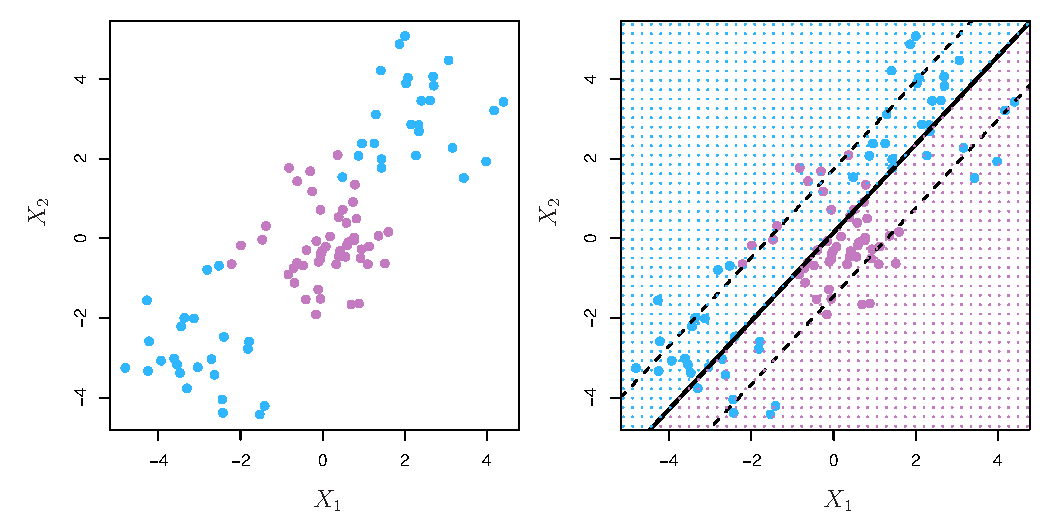
\includegraphics[trim={9.5cm 0cm 0cm 0cm}, clip, width=0.8\textwidth]{figures/9_8} \\
            \textit{\tiny A linear boundary fails to separate them.}
        \end{column}
        \begin{column}{0.4\textwidth}
            Sometime a linear boundary simply won't work, no matter what value of C. \\
            \vspace{1mm}
            The example on the left is such a case. \\
            \vspace{1mm}
            What to do?
        \end{column}
    \end{columns}
\end{frame}

\begin{frame}{Feature Expansion}
    \begin{itemize}
        \item Enlarge the space of features by including transformations; e.g. $X_{1}^{2}, X_{1}^{3}, X_{1}X_{2}, X_{1}X_{2}^{2}, \dots$ Hence go from a $p$-dimensional space to a $M > p$ dimensional space.
        \item Fit a support-vector classifier in the enlarged space.
        \item This results in non-linear decision boundaries in the original space.
    \end{itemize}
    \vspace{1em}
    \pause
    Example: Suppose we use $(X_{1}, X_{2}, X_{1}^{2}, X_{2}^{2}, X_{1}X_{2})$ instead of just $(X_{1}, X_{2})$. Then the decision boundary would be of the form
    \[ \beta_{0} + \beta_{1}X_{1} + \beta_{2}X_{2} + \beta_{3}X_{1}^{2} + \beta_{4}X_{2}^{2} + \beta_{5}X_{1}X_{2} = 0 \]
    This leads to nonlinear decision boundaries in the original space (quadratic conic sections).
\end{frame}

\begin{frame}{Cubic Polynomials}
    \begin{columns}
        \begin{column}{0.5\textwidth}
            Here we use a basis expansion of cubic polynomials. \\
            \vspace{1em}
            From 2 variables to 9. \\
            \vspace{1em}
            The support-vector classifier in the enlarged space solves the problem in the lower-dimensional space.
        \end{column}
        \begin{column}{0.5\textwidth}
            \centering
            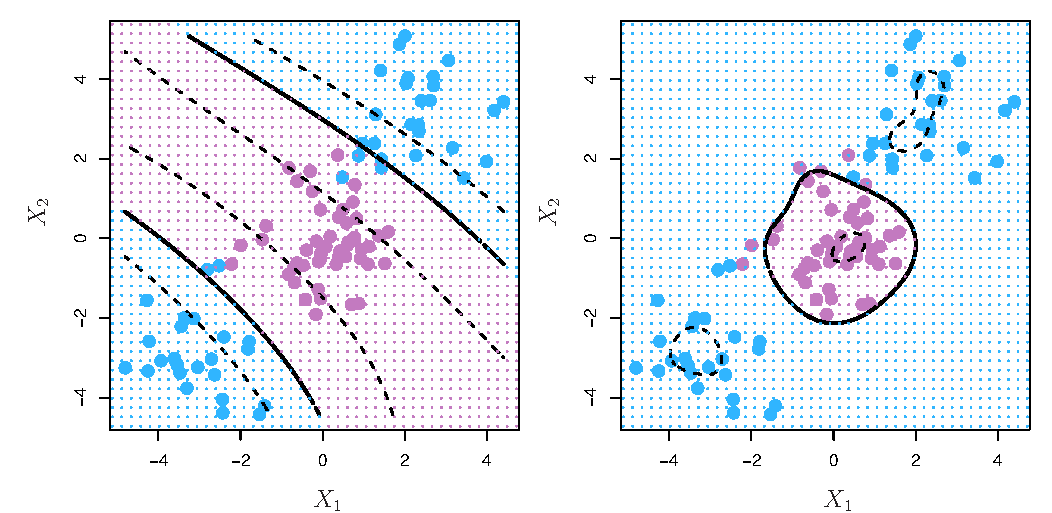
\includegraphics[trim={0cm 0cm 9cm 0cm}, clip, width=0.9\textwidth]{figures/9_9} \\
            \textit{\tiny Decision boundary of a Support Vector Classifier using a cubic polynomial kernel, successfully separating the non-linear classes.}
        \end{column}
    \end{columns}
    \pause
    {\footnotesize
    \[ \beta_{0} + \beta_{1}X_{1} + \beta_{2}X_{2} + \beta_{3}X_{1}^{2} + \beta_{4}X_{2}^{2} + \beta_{5}X_{1}X_{2} + \beta_{6}X_{1}^{3} + \beta_{7}X_{2}^{3} + \beta_{8}X_{1}X_{2}^{2} + \beta_{9}X_{1}^{2}X_{2} = 0 \]
    }
\end{frame}

\begin{frame}{Nonlinearities and Kernels}
    \begin{itemize}
        \item Polynomials (especially high-dimensional ones) get wild rather fast.
        \item There is a more elegant and controlled way to introduce nonlinearities in support-vector classifiers --- through the use of \textbf{kernels}.
        \item Before we discuss these, we must understand the role of \textbf{inner products} in support-vector classifiers.
    \end{itemize}
\end{frame}

\begin{frame}{Inner products and support vectors}
    \footnotesize
    \begin{itemize}
        \item Inner product between vectors...
        \[ \langle x_{i}, x_{i'} \rangle = \sum_{j=1}^{p} x_{ij} x_{i'j} \]
        \pause

        \item The linear support vector classifier, with \textbf{$n$ parameters}, can be represented as...
        \[ f(x) = \beta_{0} + \sum_{i=1}^{n} \alpha_{i} \langle x, x_{i} \rangle \]
        \pause

        \item To estimate the parameters $\alpha_{1}, \dots, \alpha_{n}$ and $\beta_{0}$, all we need are the $\binom{n}{2}$ inner products $\langle x_{i}, x_{i'} \rangle$ between all pairs of training observations.
    \end{itemize}

    It turns out that most of the $\hat{\alpha}_{i}$ can be zero:
    \[ f(x) = \beta_{0} + \sum_{i \in \mathcal{S}} \hat{\alpha}_{i} \langle x, x_{i} \rangle \]
    $\mathcal{S}$ is the \textbf{support set} of indices $i$ such that $\hat{\alpha}_{i} > 0$ [see slide 10]
\end{frame}

\begin{frame}{Kernels and Support Vector Machines}
    \begin{itemize}
        \item If we can compute inner-products between observations, we can fit a SV classifier. Can be quite abstract!
        \pause

        \item Some special \textbf{kernel functions} can do this for us. E.g.
        \[ K(x_{i}, x_{i'}) = \left(1 + \sum_{j=1}^{p} x_{ij} x_{i'j}\right)^{d} \]
        computes the inner-products needed for $d$ dimensional polynomials - $\binom{p+d}{d}$ basis functions! \\
        \textbf{Try it for $p=2$ and $d=2$.}
        \pause

        \item The solution has the form
        \[ f(x) = \beta_{0} + \sum_{i \in \mathcal{S}} \hat{\alpha}_{i} K(x, x_{i}). \]
    \end{itemize}
\end{frame}

\begin{frame}{Radial Kernel}
    \begin{columns}
        \begin{column}{0.5\textwidth}
            \centering
            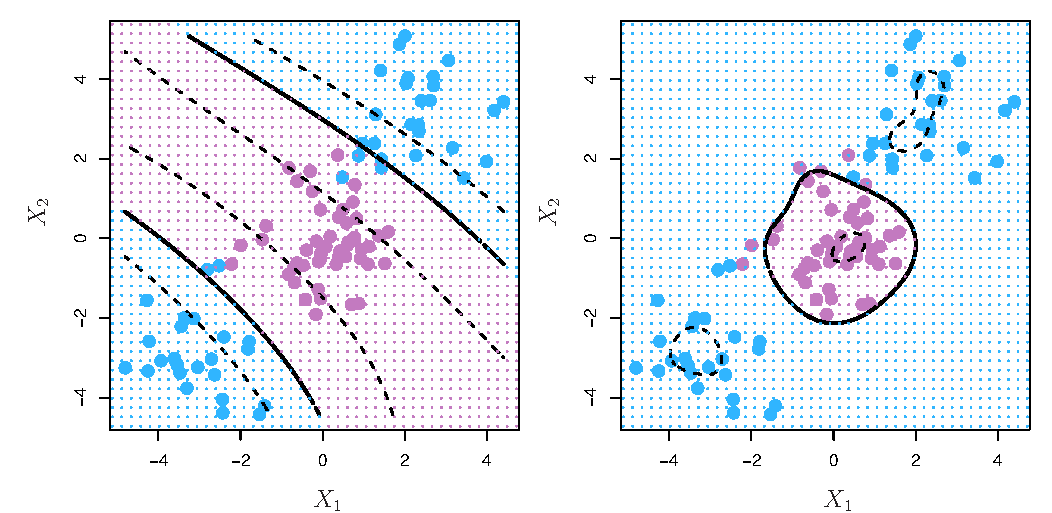
\includegraphics[trim={9.5cm 0cm 0cm 0cm}, clip, width=0.9\textwidth]{figures/9_9} \\
            \textit{\tiny Radial kernel cleanly encapsulating non-linear clusters.}
        \end{column}
        \begin{column}{0.5\textwidth}
            \[ K(x_{i}, x_{i'}) = \exp\left(-\gamma \sum_{j=1}^{p} (x_{ij} - x_{i'j})^{2}\right). \]
            \[ f(x) = \beta_{0} + \sum_{i \in \mathcal{S}} \hat{\alpha}_{i} K(x, x_{i}) \]
            Implicit feature space; very high dimensional. \\
            \vspace{1em}
            Controls variance by squashing down most dimensions severely.
        \end{column}
    \end{columns}
\end{frame}

\begin{frame}{Example: Heart Data}
    \centering
    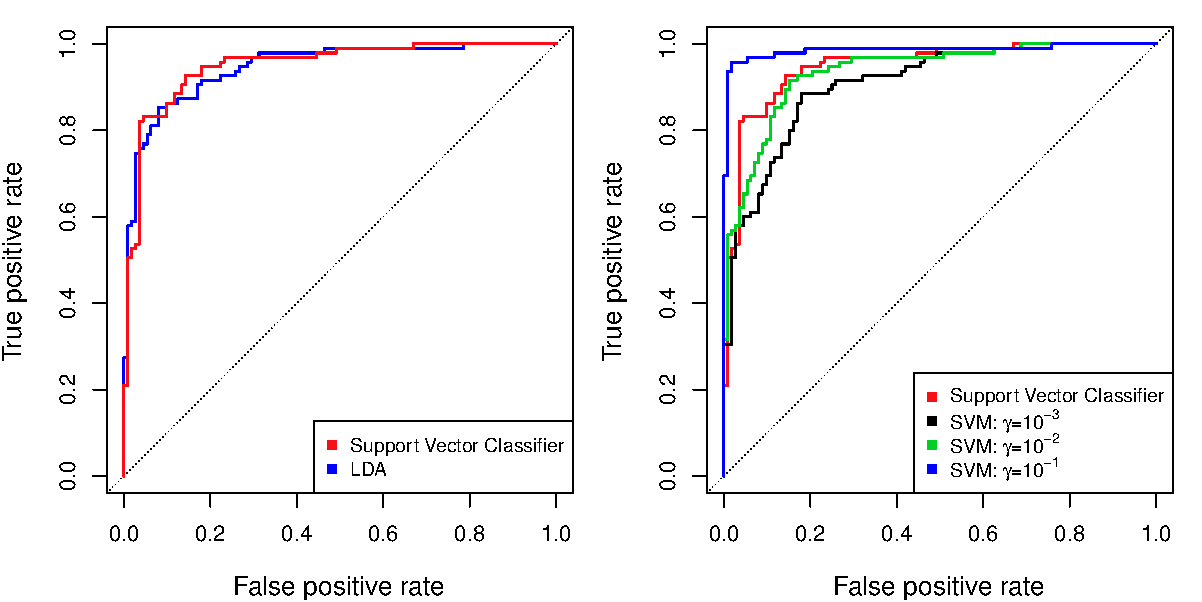
\includegraphics[width=0.8\textwidth]{figures/9_10} \\
    \textit{\tiny ROC curves on training data. LDA vs Support Vector Classifier (left). SVMs with different $\gamma$ values (right).} \\
    ROC curve is obtained by changing the threshold 0 to threshold $t$ in $\hat{f}(X) > t$ and recording \textbf{false positive} and \textbf{true positive} rates as $t$ varies. Here we see ROC curves on training data.
\end{frame}

\begin{frame}{Example continued: Heart Test Data}
    \centering
    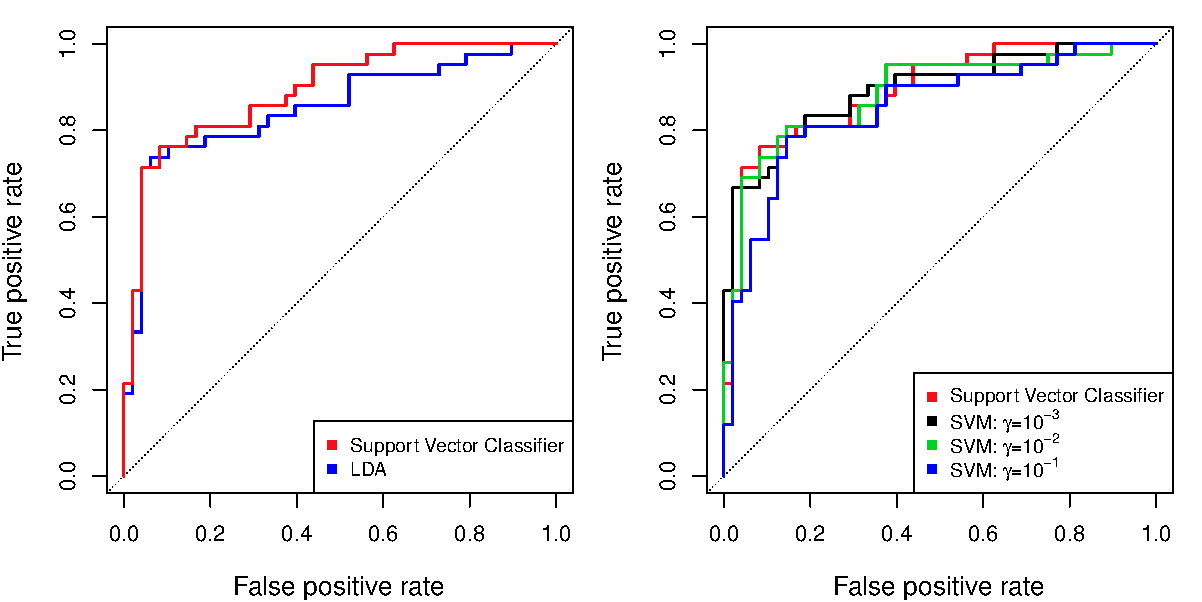
\includegraphics[width=0.8\textwidth]{figures/9_11} \\
    \textit{\tiny ROC curves on test data. LDA and Support Vector Classifier. SVMs with different $\gamma$ values ($10^{-3}, 10^{-2}, 10^{-1}$).}
\end{frame}

\begin{frame}{SVMs: more than 2 classes?}
    \begin{itemize}
        \item The SVM as defined works for $K=2$ classes. What do we do if we have $K>2$ classes?
        \pause

        \begin{itemize}
            \item \textbf{OVA} One versus All. Fit $K$ different 2-class SVM classifiers $\hat{f}_{k}(x)$, $k=1,\dots,K$; each class versus the rest. Classify $x^{*}$ to the class for which $\hat{f}_{k}(x^{*})$ is largest.
            \pause

            \item \textbf{OVO} One versus One. Fit all $\binom{K}{2}$ pairwise classifiers $\hat{f}_{kl}(x)$. Classify $x^{*}$ to the class that wins the most pairwise competitions.
            \pause

        \end{itemize}

        \item Which to choose? If $K$ is not too large, use OVO.
    \end{itemize}
\end{frame}

\begin{frame}{Support Vector versus Logistic Regression?}
    \begin{columns}
        \begin{column}{0.5\textwidth}
            \centering
            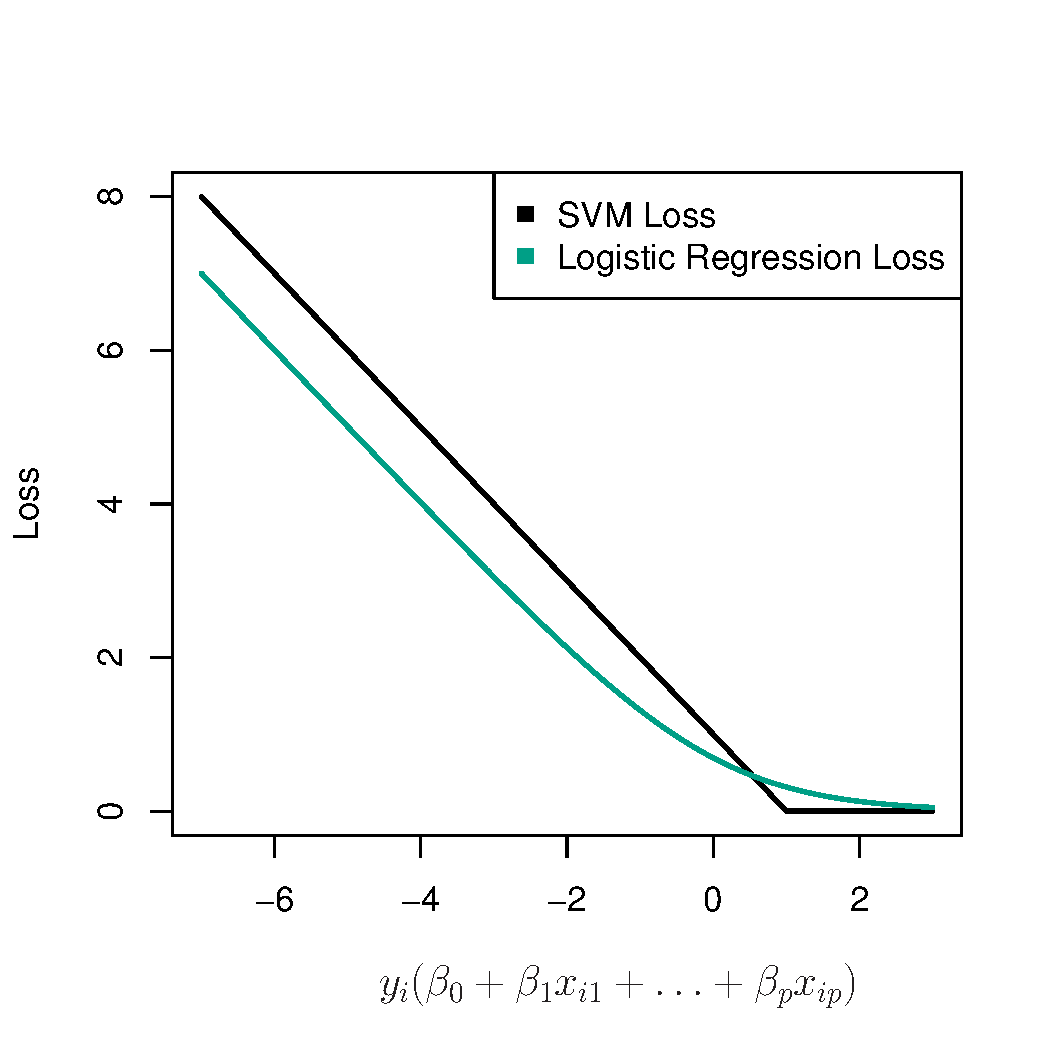
\includegraphics[width=0.9\textwidth]{figures/9_12} \\
            \textit{\tiny Line plot comparing Hinge Loss (SVM) and Negative Log-Likelihood Loss (Logistic Regression). Both look very similar.}
        \end{column}
        \begin{column}{0.5\textwidth}
            With $f(X) = \beta_{0} + \beta_{1}X_{1} + \dots + \beta_{p}X_{p}$ can rephrase support-vector classifier optimization as
            \[ \min_{\beta_{0},\beta_{1},\dots,\beta_{p}} \left\{ \sum_{i=1}^{n} \max[0, 1 - y_{i}f(x_{i})] + \lambda \sum_{j=1}^{p} \beta_{j}^{2} \right\} \]
            This has the form \textbf{loss plus penalty}. \\
            \vspace{1em}
            The loss is known as the \textbf{hinge loss}. \\
            \vspace{1em}
            Very similar to ``loss'' in logistic regression (negative log-likelihood).
        \end{column}
    \end{columns}
\end{frame}

\begin{frame}{Which to use: SVM or Logistic Regression}
    \begin{itemize}
        \item When classes are (nearly) separable, SVM does better than LR. So does LDA.
        \item When not, LR (with ridge penalty) and SVM very similar.
        \item If you wish to estimate probabilities, LR is the choice.
        \item For nonlinear boundaries, kernel SVMs are popular. Can use kernels with LR and LDA as well, but computations are more expensive.
    \end{itemize}
\end{frame}

\begin{frame}{}
    \centering
    \Huge End of Chapter 9.
\end{frame}

\begin{frame}{An Introduction to Statistical Learning with Applications in R}{a.k.a. ISLR}
    \centering
    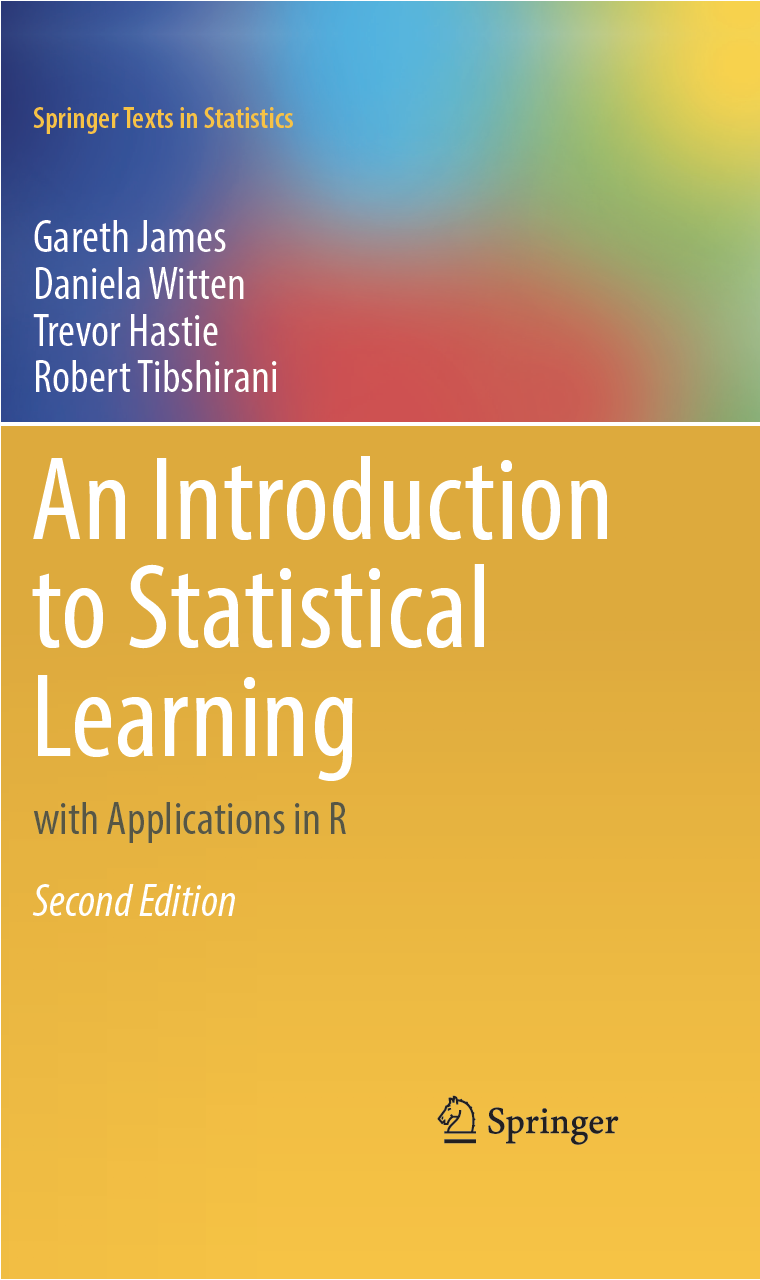
\includegraphics[height=0.7\textheight]{figures/book_cover} \\
    \vspace{4mm}
    {
        \tiny
        Content has been extracted from \textit{An Introduction to Statistical Learning with Applications in R}, Second Edition, by James, Witten, Hastie \& Tibshirani. Springer. 2023.\\
        Visit \url{https://www.statlearning.com/}.\\
    }
\end{frame}

\end{document}
